\section{\texorpdfstring{$*$}{*}Lefschetz 不动点定理}
\sourcepage{141--142}
前面的不动点定理讨论球面、球到自身的映射。Solomon Lefschetz 作出了广泛推广，使其适用于更一般的拓扑空间。本节证明这个定理。

先复习代数知识。方阵 $A=(a_{ij})$ 的\textbf{迹}（trace）定义为 $\operatorname{tr}A=\sum_{j=1}^n a_{jj}$。若 $A,B$ 都是 $n$ 阶方阵，则
\[
\operatorname{tr}(AB)=\sum_{i,j}a_{ij}b_{ji}=\operatorname{tr}(BA).
\]
若 $G$ 为基为 $e_1,\ldots,e_n$ 的自由阿贝尔群，$\varphi:G\to G$ 为同态，则定义其迹为相应矩阵的迹。它与基选择无关，因为另一组基下的矩阵为 $B^{-1}AB$，而 $\operatorname{tr}(B^{-1}(AB))=\operatorname{tr}((AB)B^{-1})=\operatorname{tr}A$。同样，若 $i$ 为同构，则 $\operatorname{tr}(i\varphi i^{-1})=\operatorname{tr}\varphi$。

设 $K$ 为有限复形，$\varphi$ 为其链复形到自身的链映射。各 $C_p(K)$ 自由有限秩，故可定义 $\operatorname{tr}(\varphi,C_p(K))$。$H_p(K)$ 不一定自由，但除去挠子群 $T_p(K)$ 后得到自由群，且 $\varphi_*$ 诱导此商群到自身的同态。以 $\operatorname{tr}(\varphi_*,H_p(K)/T_p(K))$ 表示其迹。这两个迹之间没有明显关系，所以下式相当引人注目。

\entry{定理}{2.10.1（Hopf 迹定理）}若 $K$ 为有限复形，$\varphi$ 为链映射，则
\[
\sum_p(-1)^p\operatorname{tr}(\varphi,C_p(K))
=\sum_p(-1)^p\operatorname{tr}(\varphi_*,H_p(K)/T_p(K)).
\]
\noindent\textbf{证明：第一步。}设 $G$ 自由有限秩，$H$ 为子群，且 $G/H$ 自由。若 $\varphi:G\to G$ 保持 $H$，证明
\[
\operatorname{tr}(\varphi,G)=\operatorname{tr}(\varphi',G/H)+\operatorname{tr}(\varphi'',H),
\]
其中 $\varphi',\varphi''$ 为诱导同态。选取 $G/H$ 的基 $\alpha_1+H,\ldots,\alpha_n+H$ 和 $H$ 的基 $\beta_1,\ldots,\beta_p$。若相应矩阵为 $A,B$，则
\[
\varphi'(\alpha_j+H)=\sum_i a_{ij}(\alpha_i+H),\qquad
\varphi''(\beta_j)=\sum_i b_{ij}\beta_i.
\]
$\alpha_1,\ldots,\alpha_n,\beta_1,\ldots,\beta_p$ 为 $G$ 的基，且 $\varphi(\alpha_j)=\sum_i a_{ij}\alpha_i+H\text{ 中某元素}$，$\varphi(\beta_j)=\sum_i b_{ij}\beta_i$。因此矩阵为
\[
\begin{pmatrix}A&0\\ *&B\end{pmatrix},
\]
其迹为 $\operatorname{tr}A+\operatorname{tr}B$。

\sourcepage{143--144}
\textbf{第二步。}仍以 $C_p,Z_p,B_p,W_p$ 表示链群、闭链群、边界群和弱边界群，有 $B_p\subset W_p\subset Z_p\subset C_p$。$\varphi$ 为链映射，保持这些群。将证明 $C_p/Z_p$ 与 $Z_p/W_p$ 自由，由第一步即得
\[
\operatorname{tr}(\varphi,C_p)=\operatorname{tr}(\varphi,C_p/Z_p)
+\operatorname{tr}(\varphi,Z_p/W_p)+\operatorname{tr}(\varphi,W_p).\tag{i}
\]
这里省略区分各诱导同态的撇号。

\textbf{第三步。}限制边界算子的值域，得到满同态 $C_p\to B_{p-1}$，核为 $Z_p$，故诱导同构 $C_p/Z_p\cong B_{p-1}$。后者自由，前者也自由。由于 $\varphi$ 与边界可交换，此同构与 $\varphi$ 可交换，所以
\[
\operatorname{tr}(\varphi,C_p/Z_p)=\operatorname{tr}(\varphi,B_{p-1}).\tag{ii}
\]
\textbf{第四步。}自然投影的复合 $Z_p\to Z_p/B_p=H_p\to H_p/T_p$ 为满射，核为 $W_p$，因此诱导同构 $Z_p/W_p\cong H_p/T_p$，所以前者自由。各投影与 $\varphi$ 可交换，故
\[
\operatorname{tr}(\varphi,Z_p/W_p)=\operatorname{tr}(\varphi_*,H_p/T_p).\tag{iii}
\]
\textbf{第五步。}证明
\[
\operatorname{tr}(\varphi,W_p)=\operatorname{tr}(\varphi,B_p).\tag{iv}
\]
由自由阿贝尔群基本定理，可选 $W_p$ 的基 $\alpha_1,\ldots,\alpha_n$，使 $B_p$ 有基 $m_1\alpha_1,\ldots,m_k\alpha_k$，其中 $m_i\geq1$。因为 $W_p/B_p$ 为挠群，所以 $k=n$。写作
\[
\varphi(\alpha_j)=\sum_i a_{ij}\alpha_i,\qquad
\varphi(m_j\alpha_j)=\sum_i b_{ij}(m_i\alpha_i).
\]
将前式乘以 $m_j$，比较得 $m_ja_{ij}=b_{ij}m_i$。特别地，$a_{ii}=b_{ii}$，两迹相等。

\textbf{第六步。}将 (ii)--(iv) 代入 (i)，得到
\[
\operatorname{tr}(\varphi,C_p)=\operatorname{tr}(\varphi,B_{p-1})
+\operatorname{tr}(\varphi_*,H_p/T_p)+\operatorname{tr}(\varphi,B_p).
\]
乘以 $(-1)^p$ 并对 $p$ 求和，右边第一、第三项两两抵消，即得结论。\hfill$\square$

\entry{定义}{2.10.2}有限复形 $K$ 的\textbf{Euler 数}（Euler number）经典地定义为
\[
\chi(K)=\sum_p(-1)^p\operatorname{rank}C_p(K),
\]
即各维单形数目的交错和。

\entry{定理}{2.10.3}设 $\beta_p=\operatorname{rank}(H_p(K)/T_p(K))$ 为 $p$ 维 Betti 数，则 $\chi(K)=\sum_p(-1)^p\beta_p$。

\noindent\textbf{证明：}对恒等链映射用 Hopf 迹定理。它在链群上的迹为链群的秩，在同调自由商群上的迹为 $\beta_p$。\hfill$\square$

因此 Euler 数为底空间的拓扑不变量。此定理有许多后果，例如 $\R^3$ 中有界凸开区域的边界同胚于 $S^2$，故 Euler 数为 $2$；由此可证明只有五种正多面体，即经典的五种 Platonic 立体。\translatornote{原文此处没有写出“有界”；要由凸开区域边界得到球面，需有此类限定。}

\sourcepage{145--146}
\entry{定义}{2.10.4}有限复形底空间的连续自映射 $h$ 的 \textbf{Lefschetz 数}定义为
\[
\Lambda(h)=\sum_p(-1)^p\operatorname{tr}(h_*,H_p(K)/T_p(K)).
\]
由定理 2.7.5，它只依赖同伦类。它也只依赖底空间，不依赖具体复形：若 $|L|=|K|$，恒等映射诱导同构 $j_*:H_p(L)\to H_p(K)$，而 $(h_L)_*=j_*^{-1}(h_K)_*j_*$，两者的迹相同。

\entry{定理}{2.10.5（Lefschetz 不动点定理）}若 $K$ 为有限复形，$h:|K|\to|K|$ 连续，且 $\Lambda(h)\ne0$，则 $h$ 有不动点。

\noindent\textbf{证明：}假设没有不动点，证明 $\Lambda(h)=0$。

\textbf{第一步。}可假定每个顶点 $v$ 满足
\[
h(\overline{\operatorname{St}(v,K)})\cap\overline{\operatorname{St}(v,K)}=\varnothing.\tag{$*$}
\]
令 $\epsilon=\min_x|x-h(x)|>0$。由一致连续性，选 $\delta>0$，使 $|x-y|<\delta$ 时 $|h(x)-h(y)|\leq\epsilon/3$。令 $\lambda=\min\{\delta,\epsilon/2\}$。若 $A$ 的直径小于 $\lambda$，则 $A,h(A)$ 的直径均小于 $\epsilon/2$，故必不相交。将 $K$ 换成各闭星形邻域直径小于 $\lambda$ 的剖分，$(*)$ 即成立，且 $\Lambda(h)$ 不变。

\textbf{第二步。}选剖分 $K'$，使 $h$ 有单纯逼近 $f:K'\to K$。若 $s\in K'$、$\sigma\in K$ 且 $s\subset\sigma$，断言 $f(s)\ne\sigma$。反设相等，取 $s$ 的顶点 $w$，$v=f(w)$ 为 $\sigma$ 的顶点。由 $w\in\sigma$，有 $w\in\overline{\operatorname{St}(v,K)}$，故
\[
h(w)\in h(\overline{\operatorname{St}(v,K)}).
\]
另一方面，单纯逼近条件给出 $h(\operatorname{St}(w,K'))\subset\operatorname{St}(v,K)$，故 $h(w)\in\operatorname{St}(v,K)$，与 $(*)$ 矛盾。

\textbf{第三步。}令 $\lambda:\mathcal C(K)\to\mathcal C(K')$ 为剖分算子，$\varphi=f_\#\lambda$ 诱导 $h_*$。以通常的定向单形为基，考察 $\varphi$ 的矩阵。$\lambda(\sigma)$ 为所有位于 $\sigma$ 内的定向单形 $s$ 的线性组合。由第二步，各 $f(s)$ 均不是 $\sigma$，因此 $\varphi(\sigma)$ 中 $\sigma$ 的系数为零。矩阵所有对角元都为零，故各维迹为零。由 Hopf 迹定理，$\Lambda(h)=\sum_p(-1)^p\operatorname{tr}(\varphi,C_p(K))=0$。\hfill$\square$

为应用此定理，需要下面的引理。

\entry{引理}{2.10.6}若有限复形 $K$ 的底空间连通，则任意连续自映射 $h$ 在 $H_0(K)$ 上诱导恒等映射。

\noindent\textbf{证明：}取单纯逼近 $f:K'\to K$。对顶点 $v$，剖分算子的像由 $v$ 的剖分承载，只能是 $v$ 的整数倍；保持增广迫使 $\lambda(v)=v$。所以 $f_\#\lambda(v)=f_\#(v)$ 为一个顶点，由连通性，它同调于 $v$。故 $h_*$ 为恒等映射。\translatornote{原文证明首句将 $f$ 的目标误写为 $K'$，这里取 $K$。}\hfill$\square$

\entry{定理}{2.10.7}若有限复形底空间无环，则其每个连续自映射都有不动点。

\noindent\textbf{证明：}$H_0(K)\cong\Z$，且其上 $h_*$ 为恒等映射，迹为 $1$。高维同调为零，故 $\Lambda(h)=1$，定理适用。\hfill$\square$

\sourcepage{147--149}
\entry{定理}{2.10.8}对径映射 $a:S^n\to S^n$ 的度为 $(-1)^{n+1}$。

\noindent\textbf{证明：}若 $h$ 的度为 $d$，则零维同调上的迹为 $1$，最高维同调上的迹为 $d$，故
\[
\Lambda(h)=1+(-1)^n d.\tag{$\dagger$}
\]
对径映射无不动点，所以 $\Lambda(a)=0$，即 $1+(-1)^n\deg a=0$，得到结论。\hfill$\square$

下列定义用于习题 6。

\entry{定义}{2.10.9}设 $\mathcal B$ 是 $\R^3$ 中的有限多边形族，任意两者至多相交于一条公共边或一个公共顶点。各多边形称为 $\mathcal B$ 的\textbf{面}，其边、顶点分别称为 $\mathcal B$ 的边、顶点。若每个面有相同边数 $k$，每条边恰属于两个面，每个顶点恰属于相同数目 $\ell$ 的面，则称 $\mathcal B$ \textbf{组合正则}（combinatorially regular）。四面体边界的三角形族和立方体边界的正方形族都是例子。

\subsection*{习题}
\begin{enumerate}
\item 证明每个映射 $f:P^2\to P^2$ 都有不动点。
\item 并非每个 $S^0$ 到自身的连续映射都有不动点，$S^1$ 也如此，验证这些断言。对 $S^2$ 的连续自映射能说些什么？
\item 若有限复形的自映射 $h$ 同伦于常值映射，证明 $h$ 有不动点。
\item \begin{enumerate}[label=(\alph*)]
\item 证明存在 Klein 瓶的自映射 $f$，将图 2.10.1 的曲线 $C$ 同胚地映到 $D$，并存在自映射 $g$ 将 $C$ 映入阴影区域 $E$。
\begin{center}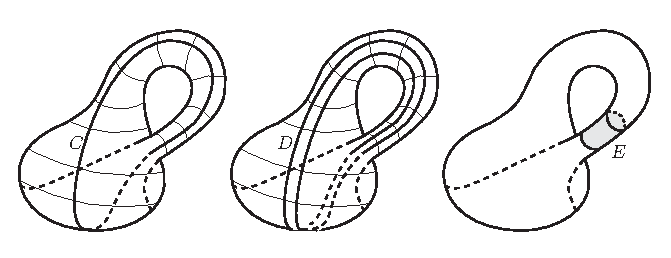
\includegraphics[width=118mm]{figures/2-10-1.pdf}\\图 2.10.1\end{center}
\item 若 $f\simeq f'$、$g\simeq g'$，证明 $f',g'$ 都有不动点。
\item 找出一个没有不动点的 Klein 瓶自映射。
\end{enumerate}
\item 设 $M$ 为 $\R^n$ 中的紧致光滑曲面，$v(x)$ 为切向量场。微分几何的标准结果说明：存在 $\epsilon>0$ 及连续映射 $F:M\times(-\epsilon,\epsilon)\to M$，使曲线 $t\mapsto F(x_0,t)$ 在 $t=0$ 经过 $x_0$，速度为 $v(x_0)$。若 $v$ 处处非零，则存在 $\delta>0$，使对所有 $x_0$ 和 $0<|t|<\delta$，都有 $F(x_0,t)\ne x_0$。
\begin{enumerate}[label=(\alph*)]
\item 利用这些事实，证明若 $M$ 有处处非零的切向量场，则 $\chi(M)=0$。
\item 确定哪些紧致曲面有处处非零的切向量场。
\end{enumerate}
\item 设多边形族 $\mathcal B$ 如定义 2.10.9。
\begin{enumerate}[label=(\alph*)]
\item 以 $|\mathcal B|$ 表示各多边形的并，证明 $\chi(\mathcal B)=\text{面数}-\text{边数}+\text{顶点数}$。［提示：从每个面的内点作星形剖分，得到单纯复形。］
\item 证明底空间同胚于 $S^2$ 的组合正则族只有五种。［提示：几何条件给出 $k\geq3$、$\ell\geq3$。］\translatornote{这里应按组合类型理解“五种”，并非指其在 $\R^3$ 中只有五种具体几何嵌入。}
\item 底空间同胚于环面的组合正则族有许多，但 $k,\ell$ 的可能值有限，求这些可能值。
\end{enumerate}
\item 设 $B\subset\R^N$ 为开单位球，举出没有不动点的连续自映射；再举出同时为一一且满的例子。
\item 设 $B^N$ 为闭单位球，举出不连续且没有不动点的自映射。
\item 令 $S=\{(\cos t,\sin t,t):0\leq t\leq4\pi\}$，$E=\{x\in\R^3:\operatorname{dist}(x,S)\leq1/10\}$，证明每个连续映射 $f:E\to E$ 都有不动点。
\end{enumerate}
